% Generated by ArticleSignalDiagrams. Opaque vector fills only.
\documentclass[10pt,tikz,border=5pt]{standalone}
\usepackage{lmodern}
\usetikzlibrary{fit}
\begin{document}
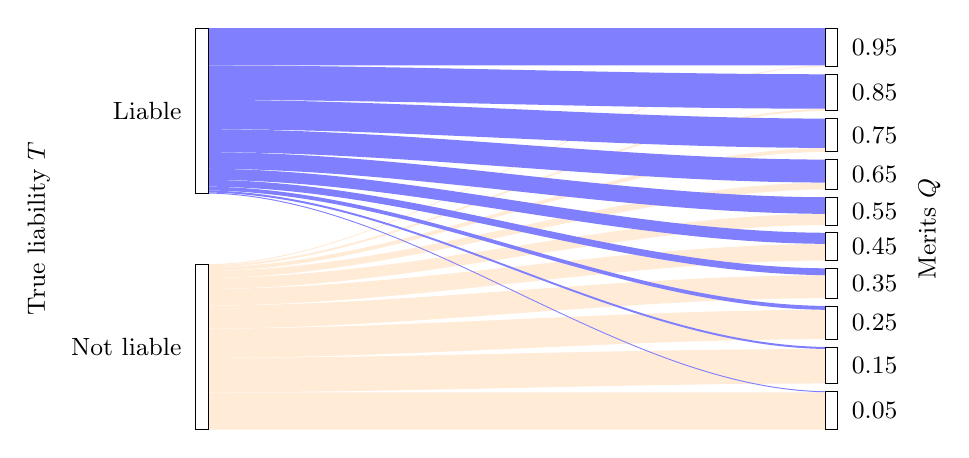
\begin{tikzpicture}[x=1cm,y=1cm,font=\small]\path[fill=orange!16!white,draw=none] (3.3,-5.1) .. controls (6,-5.1) and (8.6,-5.1) .. (11.3,-5.1) -- (11.3,-4.625676) .. controls (8.6,-4.625676) and (6,-4.625676) .. (3.3,-4.625676) -- cycle;
\path[fill=orange!16!white,draw=none] (3.3,-4.625676) .. controls (6,-4.625676) and (8.6,-4.513332) .. (11.3,-4.513332) -- (11.3,-4.075947) .. controls (8.6,-4.075947) and (6,-4.188292) .. (3.3,-4.188292) -- cycle;
\path[fill=orange!16!white,draw=none] (3.3,-4.188292) .. controls (6,-4.188292) and (8.6,-3.950338) .. (11.3,-3.950338) -- (11.3,-3.578427) .. controls (8.6,-3.578427) and (6,-3.816381) .. (3.3,-3.816381) -- cycle;
\path[fill=orange!16!white,draw=none] (3.3,-3.816381) .. controls (6,-3.816381) and (8.6,-3.429436) .. (11.3,-3.429436) -- (11.3,-3.137827) .. controls (8.6,-3.137827) and (6,-3.524772) .. (3.3,-3.524772) -- cycle;
\path[fill=orange!16!white,draw=none] (3.3,-3.524772) .. controls (6,-3.524772) and (8.6,-2.951408) .. (11.3,-2.951408) -- (11.3,-2.740569) .. controls (8.6,-2.740569) and (6,-3.313933) .. (3.3,-3.313933) -- cycle;
\path[fill=orange!16!white,draw=none] (3.3,-3.313933) .. controls (6,-3.313933) and (8.6,-2.5) .. (11.3,-2.5) -- (11.3,-2.359431) .. controls (8.6,-2.359431) and (6,-3.173364) .. (3.3,-3.173364) -- cycle;
\path[fill=orange!16!white,draw=none] (3.3,-3.173364) .. controls (6,-3.173364) and (8.6,-2.048592) .. (11.3,-2.048592) -- (11.3,-1.962173) .. controls (8.6,-1.962173) and (6,-3.086945) .. (3.3,-3.086945) -- cycle;
\path[fill=orange!16!white,draw=none] (3.3,-3.086945) .. controls (6,-3.086945) and (8.6,-1.570564) .. (11.3,-1.570564) -- (11.3,-1.521573) .. controls (8.6,-1.521573) and (6,-3.037954) .. (3.3,-3.037954) -- cycle;
\path[fill=orange!16!white,draw=none] (3.3,-3.037954) .. controls (6,-3.037954) and (8.6,-1.049662) .. (11.3,-1.049662) -- (11.3,-1.024053) .. controls (8.6,-1.024053) and (6,-3.012344) .. (3.3,-3.012344) -- cycle;
\path[fill=orange!16!white,draw=none] (3.3,-3.012344) .. controls (6,-3.012344) and (8.6,-0.486668) .. (11.3,-0.486668) -- (11.3,-0.474324) .. controls (8.6,-0.474324) and (6,-3) .. (3.3,-3) -- cycle;
\path[fill=blue!50!white,draw=none] (3.3,-2.1) .. controls (6,-2.1) and (8.6,-4.625676) .. (11.3,-4.625676) -- (11.3,-4.613332) .. controls (8.6,-4.613332) and (6,-2.087656) .. (3.3,-2.087656) -- cycle;
\path[fill=blue!50!white,draw=none] (3.3,-2.087656) .. controls (6,-2.087656) and (8.6,-4.075947) .. (11.3,-4.075947) -- (11.3,-4.050338) .. controls (8.6,-4.050338) and (6,-2.062046) .. (3.3,-2.062046) -- cycle;
\path[fill=blue!50!white,draw=none] (3.3,-2.062046) .. controls (6,-2.062046) and (8.6,-3.578427) .. (11.3,-3.578427) -- (11.3,-3.529436) .. controls (8.6,-3.529436) and (6,-2.013055) .. (3.3,-2.013055) -- cycle;
\path[fill=blue!50!white,draw=none] (3.3,-2.013055) .. controls (6,-2.013055) and (8.6,-3.137827) .. (11.3,-3.137827) -- (11.3,-3.051408) .. controls (8.6,-3.051408) and (6,-1.926636) .. (3.3,-1.926636) -- cycle;
\path[fill=blue!50!white,draw=none] (3.3,-1.926636) .. controls (6,-1.926636) and (8.6,-2.740569) .. (11.3,-2.740569) -- (11.3,-2.6) .. controls (8.6,-2.6) and (6,-1.786067) .. (3.3,-1.786067) -- cycle;
\path[fill=blue!50!white,draw=none] (3.3,-1.786067) .. controls (6,-1.786067) and (8.6,-2.359431) .. (11.3,-2.359431) -- (11.3,-2.148592) .. controls (8.6,-2.148592) and (6,-1.575228) .. (3.3,-1.575228) -- cycle;
\path[fill=blue!50!white,draw=none] (3.3,-1.575228) .. controls (6,-1.575228) and (8.6,-1.962173) .. (11.3,-1.962173) -- (11.3,-1.670564) .. controls (8.6,-1.670564) and (6,-1.283619) .. (3.3,-1.283619) -- cycle;
\path[fill=blue!50!white,draw=none] (3.3,-1.283619) .. controls (6,-1.283619) and (8.6,-1.521573) .. (11.3,-1.521573) -- (11.3,-1.149662) .. controls (8.6,-1.149662) and (6,-0.911708) .. (3.3,-0.911708) -- cycle;
\path[fill=blue!50!white,draw=none] (3.3,-0.911708) .. controls (6,-0.911708) and (8.6,-1.024053) .. (11.3,-1.024053) -- (11.3,-0.586668) .. controls (8.6,-0.586668) and (6,-0.474324) .. (3.3,-0.474324) -- cycle;
\path[fill=blue!50!white,draw=none] (3.3,-0.474324) .. controls (6,-0.474324) and (8.6,-0.474324) .. (11.3,-0.474324) -- (11.3,-0) .. controls (8.6,-0) and (6,0) .. (3.3,0) -- cycle;
\coordinate (axis-midline-0) at (0,-2.55);
\path[fill=white,draw=black,line width=0.3pt] (3.22,-5.1) rectangle (3.38,-3);
\node[anchor=east,fill=white,inner sep=2pt] (bucket-0-0-0) at (3.12,-4.05) {Not liable};
\path[fill=white,draw=black,line width=0.3pt] (3.22,-2.1) rectangle (3.38,0);
\node[anchor=east,fill=white,inner sep=2pt] (bucket-0-0-1) at (3.12,-1.05) {Liable};
\node[fit=(bucket-0-0-0) (bucket-0-0-1),inner sep=0pt] (source-labels-0) {};
\coordinate (axis-title-0-0) at (source-labels-0.west |- axis-midline-0);
\node[rotate=90,anchor=south,inner sep=0pt] at ([xshift=-0.18cm]axis-title-0-0) {True liability $T$};
\path[fill=white,draw=black,line width=0.3pt] (11.22,-5.1) rectangle (11.38,-4.613332);
\node[anchor=west,fill=white,inner sep=2pt] (bucket-0-1-0) at (11.48,-4.856666) {0.05};
\path[fill=white,draw=black,line width=0.3pt] (11.22,-4.513332) rectangle (11.38,-4.050338);
\node[anchor=west,fill=white,inner sep=2pt] (bucket-0-1-1) at (11.48,-4.281835) {0.15};
\path[fill=white,draw=black,line width=0.3pt] (11.22,-3.950338) rectangle (11.38,-3.529436);
\node[anchor=west,fill=white,inner sep=2pt] (bucket-0-1-2) at (11.48,-3.739887) {0.25};
\path[fill=white,draw=black,line width=0.3pt] (11.22,-3.429436) rectangle (11.38,-3.051408);
\node[anchor=west,fill=white,inner sep=2pt] (bucket-0-1-3) at (11.48,-3.240422) {0.35};
\path[fill=white,draw=black,line width=0.3pt] (11.22,-2.951408) rectangle (11.38,-2.6);
\node[anchor=west,fill=white,inner sep=2pt] (bucket-0-1-4) at (11.48,-2.775704) {0.45};
\path[fill=white,draw=black,line width=0.3pt] (11.22,-2.5) rectangle (11.38,-2.148592);
\node[anchor=west,fill=white,inner sep=2pt] (bucket-0-1-5) at (11.48,-2.324296) {0.55};
\path[fill=white,draw=black,line width=0.3pt] (11.22,-2.048592) rectangle (11.38,-1.670564);
\node[anchor=west,fill=white,inner sep=2pt] (bucket-0-1-6) at (11.48,-1.859578) {0.65};
\path[fill=white,draw=black,line width=0.3pt] (11.22,-1.570564) rectangle (11.38,-1.149662);
\node[anchor=west,fill=white,inner sep=2pt] (bucket-0-1-7) at (11.48,-1.360113) {0.75};
\path[fill=white,draw=black,line width=0.3pt] (11.22,-1.049662) rectangle (11.38,-0.586668);
\node[anchor=west,fill=white,inner sep=2pt] (bucket-0-1-8) at (11.48,-0.818165) {0.85};
\path[fill=white,draw=black,line width=0.3pt] (11.22,-0.486668) rectangle (11.38,-0);
\node[anchor=west,fill=white,inner sep=2pt] (bucket-0-1-9) at (11.48,-0.243334) {0.95};
\node[fit=(bucket-0-1-0) (bucket-0-1-1) (bucket-0-1-2) (bucket-0-1-3) (bucket-0-1-4) (bucket-0-1-5) (bucket-0-1-6) (bucket-0-1-7) (bucket-0-1-8) (bucket-0-1-9),inner sep=0pt] (destination-labels-0) {};
\coordinate (axis-title-0-1) at (destination-labels-0.east |- axis-midline-0);
\node[rotate=90,anchor=north,inner sep=0pt] at ([xshift=0.18cm]axis-title-0-1) {Merits $Q$};
\end{tikzpicture}
\end{document}

